\documentclass{beamer}

% Beamer style
%\usetheme[secheader]{Madrid}
\usetheme{CambridgeUS}
\usecolortheme[rgb={0.65,0.15,0.25}]{structure}
%\usefonttheme[onlymath]{serif}
\beamertemplatenavigationsymbolsempty
%\AtBeginSubsection

% Packages
%\usepackage[french]{babel}
\usepackage[latin1]{inputenc}
\usepackage{color}
\usepackage{dsfont, stmaryrd}
\usepackage{amsmath, amsfonts, amssymb}
\usepackage{stmaryrd}
\usepackage{epsfig}
\usepackage{url}
\usepackage{/Latex/astats}
%\usepackage[all]{xy}
\usepackage{graphicx}

% Commands
\definecolor{darkred}{rgb}{0.65,0.15,0.25}
\newcommand{\emphase}[1]{\textcolor{darkred}{#1}}
\newcommand{\paragraph}[1]{\emphase{#1}}
\newcommand{\refer}[1]{\textcolor{blue}{\sl \cite{#1}}}
\newcommand{\Refer}[1]{\textcolor{blue}{\sl #1}}
\newcommand{\newblock}{}

% Symbols
\newcommand{\Acal}{\mathcal{A}}
\newcommand{\Abf}{{\bf A}}
\newcommand{\Beta}{\text{B}}
\newcommand{\Bcal}{\mathcal{B}}
\newcommand{\BIC}{\text{BIC}}
\newcommand{\dd}{\text{d}}
\newcommand{\dbf}{{\bf d}}
\newcommand{\Dcal}{\mathcal{D}}
\newcommand{\Esp}{\mathbb{E}}
\newcommand{\Ecal}{\mathcal{E}}
\newcommand{\Gcal}{\mathcal{G}}
\newcommand{\Gam}{\mathcal{G}\mbox{am}}
\newcommand{\Ibb}{\mathbb{I}}
\newcommand{\Ibf}{{\bf I}}
\newcommand{\Ical}{\mathcal{I}}
\newcommand{\ICL}{\text{ICL}}
\newcommand{\Cov}{\mathbb{C}\text{ov}}
\newcommand{\Corr}{\mathbb{C}\text{orr}}
\newcommand{\Var}{\mathbb{V}}
\newcommand{\Vsf}{\mathsf{V}}
\newcommand{\pen}{\text{pen}}
\newcommand{\Fcal}{\mathcal{F}}
\newcommand{\Hbf}{{\bf H}}
\newcommand{\Hcal}{\mathcal{H}}
\newcommand{\Jcal}{\mathcal{J}}
\newcommand{\Kbf}{{\bf K}}
\newcommand{\Lcal}{\mathcal{L}}
\newcommand{\Mcal}{\mathcal{M}}
\newcommand{\mbf}{{\bf m}}
\newcommand{\mum}{\mu(\mbf)}
\newcommand{\Ncal}{\mathcal{N}}
\newcommand{\Nbf}{{\bf N}}
\newcommand{\Nm}{N(\mbf)}
\newcommand{\Ocal}{\mathcal{O}}
\newcommand{\Obf}{{\bf 0}}
\newcommand{\Omegas}{\underset{s}{\Omega}}
\newcommand{\Pbf}{{\bf P}}
\newcommand{\Pcal}{\mathcal{P}}
\newcommand{\Qcal}{\mathcal{Q}}
\newcommand{\Rbb}{\mathbb{R}}
\newcommand{\Rcal}{\mathcal{R}}
\newcommand{\sbf}{{\bf s}}
\newcommand{\Sbf}{{\bf S}}
\newcommand{\Scal}{\mathcal{S}}
\newcommand{\Ucal}{\mathcal{U}}
\newcommand{\Vcal}{\mathcal{V}}
\newcommand{\Tbf}{{\bf T}}
\newcommand{\ubf}{{\bf u}}
\newcommand{\Ubf}{{\bf U}}
\newcommand{\Wbf}{{\bf W}}
\newcommand{\xbf}{{\bf x}}
\newcommand{\Xbf}{{\bf X}}
\newcommand{\ybf}{{\bf y}}
\newcommand{\Ybf}{{\bf Y}}
\newcommand{\zbf}{{\bf z}}
\newcommand{\Zbf}{{\bf Z}}
\newcommand{\betabf}{\mbox{\mathversion{bold}{$\beta$}}}
\newcommand{\pibf}{\mbox{\mathversion{bold}{$\pi$}}}
\newcommand{\Sigmabf}{\mbox{\mathversion{bold}{$\Sigma$}}}
\newcommand{\gammabf}{\mbox{\mathversion{bold}{$\gamma$}}}
\newcommand{\mubf}{\mbox{\mathversion{bold}{$\mu$}}}
\newcommand{\nubf}{\mbox{\mathversion{bold}{$\nu$}}}
\newcommand{\Thetabf}{\mbox{\mathversion{bold}{$\Theta$}}}
\newcommand{\thetabf}{\mbox{\mathversion{bold}{$\theta$}}}
\newcommand{\BP}{\text{BP}}
\newcommand{\EM}{\text{EM}}
\newcommand{\VEM}{\text{VEM}}
\newcommand{\VBEM}{\text{VB}}
\newcommand{\cst}{\text{cst}}
\newcommand{\obs}{\text{obs}}
\newcommand{\ra}{\emphase{ $\rightarrow$~}}
\newcommand{\QZ}{Q_{Z}}
\newcommand{\Qt}{Q_{\theta}}

% Directory
\newcommand{\fignet}{/RECHERCHE/RESEAUX/Exposes/Figures}
\newcommand{\figmotif}{/RECHERCHE/RESEAUX/Motifs/FIGURES}


%====================================================================
\title[Estimating Species Abundance]{Estimating Species Abundance. \\
  Application to Metagenomics}

\author[S. Robin]{S. Li-Thiao-T�, J.-J. Daudin, \underline{S. Robin}}

\institute[AgroParisTech / INRA]{AgroParisTech / INRA \\
  \bigskip
  \begin{tabular}{ccccc}
    
\epsfig{file=../Figures/LogoINRA-Couleur.ps, width=2.5cm} &
    \hspace{.5cm} &
    
\epsfig{file=../Figures/logagroptechsolo.eps, width=3.75cm} &
    \hspace{.5cm} &
    \epsfig{file=../Figures/Logo-SSB.eps, width=2.5cm} \\
  \end{tabular} \\
  \bigskip
  }

\date[LIX Colloquium, 11/2010]{LIX Bioinformatics Colloquium, November
  2010}
%====================================================================

%====================================================================
%====================================================================
\begin{document}
%====================================================================
%====================================================================

%====================================================================
\frame{\titlepage}
%====================================================================

% %====================================================================
% \frame{ \frametitle{Outline}
% %====================================================================
  
%   \setcounter{tocdepth}{1}
%   \tableofcontents
% %  \tableofcontents[pausesections]
%   }

%====================================================================
\section{Species abundance}
\frame{ \frametitle{Species abundance}}
%====================================================================

%====================================================================
\subsection{Metagenomics}
\frame{ \frametitle{Bacterial communities}
%====================================================================
  \paragraph{Biological context:} Many bacterial species can not be
  grown artificially out of their natural middle, mostly because of
  vital interactions between them.
  
  \bigskip   
  Such species can only be studied all together, within their middle,
  e.g.
  $$
  \text{Ocean, \quad Human gut, \quad Soil, \quad Cheese surface, \quad etc}
  $$

  \bigskip\pause
  \paragraph{Their diversity and functions} can be studied via NGS by
  sampling and sequencing DNA (or RNA) from \emphase{all species} 
%   \begin{itemize}
%   \item simultaneously,
%   \item sometimes without knowing who is who,
%   \item sometimes without most genome sequences.
%   \end{itemize}\pause
%   \ra '\emphase{What's in the mix?}' (\refer{McR07})
  \begin{itemize}
  \item '\emphase{What's in the mix?}' (\refer{McR07})
  \item Or, most modestly, \emphase{how many species are there?}
  \end{itemize}
  }

%====================================================================
\frame{ \frametitle{How many species are there?} 
  \paragraph{An old ecological problem} when exploring a given middle:
  how many species are not observed? \\

  \begin{tabular}{ll}
    \hspace{-.5cm}
    \begin{tabular}{p{.5\textwidth}}
      \begin{itemize}
      \item $X_i = $ number of observed individuals from species $i$,
      \item $C_x = $ number of species with $x$ observed individuals,
%         $$
%         C_x = \sum_i \Ibb\{X_i = x\},
%         $$
      \item $C = $ total number of species $= \sum_{x\geq 0} C_x$.
      \end{itemize}
      \emphase{Problem: $\widehat{C}_0 = ?$, $\widehat{C} = ?$}
    \end{tabular}
    &
    \hspace{-.5cm} \pause
    \begin{tabular}{p{.5\textwidth}}
%       \centerline{$C_x = f(x)$} 
      \vspace{-.5cm}
      \epsfig{file = ../Figures/FCW43-Fig1.ps, width=.45\textwidth,
        clip=}
      \vspace{-.5cm}
      \refer{FCW43}
    \end{tabular}
  \end{tabular}

  \bigskip\pause
  \paragraph{Metagenomics:} 
  \begin{itemize}
  \item $X_i =$ number of reads from \emphase{species $i$} (if the
    genome is available)
  \item $X_i =$ number of reads from \emphase{gene $i$} (whatever the species)
  \end{itemize}
  }

%====================================================================
\subsection{Species abundance distribution (SAD)}
\frame{ \frametitle{Species abundance distribution}
%==================================================================== 
  \paragraph{General strategy:} The observed counts $\{X_i\}$ are
  truncated, meaning that 0's are not observed. 
  \begin{enumerate} 
  \item Suppose that the 'complete' counts are i.i.d., with
    distribution $F$:
    $$
    \emphase{F = \text{species abundance distribution (SAD)}};
    $$
  \item The observed counts $\{X_i\}$ are i.i.d. with \emphase{truncated
    SAD $F_+$}
    $$
    f_+(x) = \frac{f(x)}{1- f(0)} \qquad \text{for } x =1, 2, \dots;
    $$
  \item Fit some (parametric?) distribution to the $\{X_i\}$ \ra
    $\widehat{f}_+(\cdot) = f_+(\cdot; \widehat{\gamma})$;
  \item Estimate $f(0)$ as $\widehat{f}(0) = f(0; \widehat{\gamma})$
    and $C$ as
    $$
    \widehat{C} = c \left/ [1 - \widehat{f}(0)]\right.
    $$
    known as the \emphase{Horwitz-Thomson estimate}.
  \end{enumerate}
  }

%====================================================================
\frame{ \frametitle{Statistical questions}
  
  \begin{tabular}{ll}
    \hspace{-.5cm}
    \begin{tabular}{p{.4\textwidth}}
      \paragraph{Our goal} is to
      \begin{itemize}
      \item Provide an \emphase{estimate of $C$}
      \item With \emphase{confidence bounds}.
      \end{itemize}
    \end{tabular}
    & 
    \hspace{-.5cm}
    \begin{tabular}{p{.6\textwidth}}
%       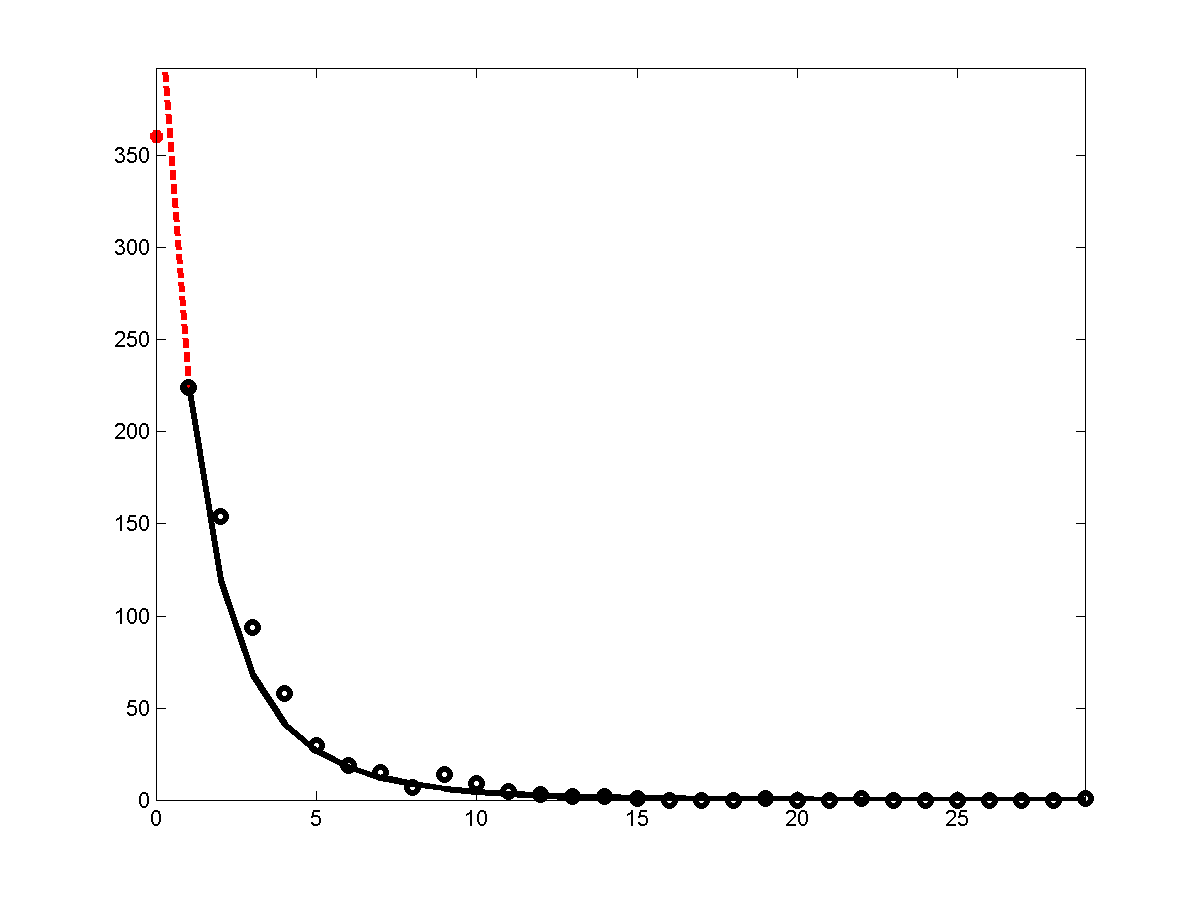
\includegraphics[width=0.5\textwidth,
%       height=0.5\textheight]{../Figures/SimMixtGeom.pdf} 
       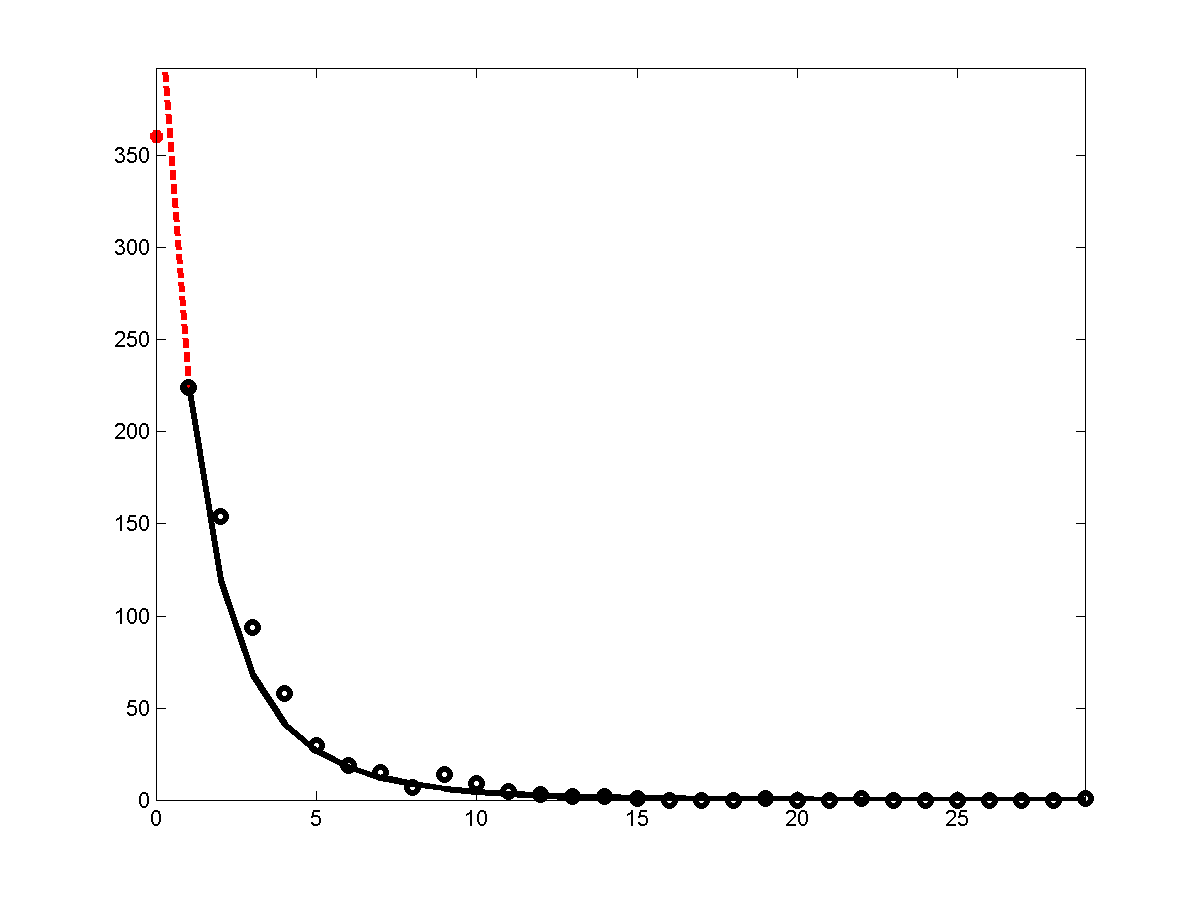
\epsfig{file=../Figures/SimMixtGeom.eps, 
       width=.45\textwidth, height=.4\textheight, clip=} 
    \end{tabular}
  \end{tabular}  
  \pause
  \paragraph{Interest of the SAD:} 
  \begin{itemize}
  \item Modelling the SAD allows to constrain on $F$, to
    \emphase{guaranty identifiability}.
  \item The SAD also help to draw the \emphase{saturation curve} to
    calibrate experiments:
    $$
    \Pr\{X_i > 0\} = \text{f(total number of observed individuals}).
    $$
  \end{itemize}
  }

%====================================================================
\section{Modelling the SAD}
\frame{ \frametitle{Modelling the SAD}}
%==================================================================== 

%====================================================================
\subsection{Fisher's model}
\frame{ \frametitle{Modelling the SAD}
%==================================================================== 
  Very little is known about the shape of $f$, so we need a flexible
  modelling.
  \begin{itemize}
  \item \paragraph{Poisson} $P = \Pcal(\lambda)$ \pause
  \item \paragraph{Log-normal } $P = \Lcal\Ncal(\mu,
    \sigma^2) $ (\refer{DoB08}) \pause
  \item \paragraph{Reference model: Poisson-Gamma} (\refer{FCW43},
    \refer{HDP10})
    $$
    \{\Lambda_i\} \text{ i.i.d.} \sim \Gam, 
    \qquad
    \{X_i\} \text{ independent } X_i \sim \Pcal(\Lambda_i).
    $$
    $$
    f(x) = \int e^{-\lambda} \frac{\lambda^x}{x!} g(\lambda) \dd \lambda
    $$
    where $g(\lambda)$ is the Gamma density. \pause
  \item \paragraph{Generalisation:} The counts are distributed
    according to some discrete distribution $\phi(\cdot; \gamma)$
    conditionally on $\gamma$:
    $$
    f(x) = \int \phi(x; \gamma) g(\gamma) \dd \gamma
    $$
    where $g(\gamma)$ is some distribution of the parameter space.
  \end{itemize}

    }

%====================================================================
\frame{ \frametitle{'Non-parametric' framework} 
  \paragraph{'Non-parametric' = mixture of Dirac masses:} \refer{NoP98}
  $$
  g(\gamma) = \sum_k \pi_k \delta_{\gamma_k}(\gamma) \quad \Rightarrow \quad
  f(x) = \int \phi(x; \gamma) g(\gamma) \dd \gamma = \sum_k \pi_k \phi(x;
  \gamma_k).
  $$

  \bigskip\pause
  \paragraph{Truncated mixture vs Mixture of truncated.} The
  distribution of the observed counts can be expressed in \emphase{two
    equivalent ways}:
  \begin{eqnarray}
    f_+(x) & = & \sum_k \pi_k \phi(x; \gamma_k) \left/ \left[ 1 -
        \sum_k \pi_k \phi(0; \gamma_k) \right]
        \right. \label{Eq:TruncMixt} \\
    \text{or} \qquad f_+(x) & = & \sum_k \emphase{\pi^+_k \phi_+}(x;
        \gamma_k). \label{Eq:MixtTrunc} 
  \end{eqnarray}

  }

%====================================================================
\frame{ \frametitle{Incomplete data model}
  
  A mixture model can be rewritten as:
  \begin{eqnarray*}
    (Z_i)_i \text{ i.i.d.:} \quad Z_i & \sim & \Mcal(1; \pibf), \\
    (X_i)_i \text{ indep. } | (Z_i)_i: \quad X_i|Z_i=k & \sim &
    \phi_+(\cdot; \gamma_k)
  \end{eqnarray*}
  where $Z_i$ is the \emphase{unknown group to which species $i$
    belongs}. 

  \bigskip
  \begin{tabular}{cc}
    \hspace{-.5cm}
    \begin{tabular}{p{.5\textwidth}}
      \paragraph{Notations:}
      \begin{eqnarray*}
        \Xbf = (X_i)_i &  & \text{the \emphase{observed} counts}, \\
        \Zbf = (Z_i)_i &  & \text{the \emphase{unobserved} groups} \\
        \thetabf = (\pibf, \gammabf) &  & \text{the
          \emphase{parameter}}
%        : \pibf = (\pi_k)_k, \; \gammabf =
        (\gamma_k)_k.  
      \end{eqnarray*}
      
      \medskip\pause
      \begin{itemize}
      \item We need get an \emphase{estimate $\widehat{\thetabf}$}
      \item or to calculate the \emphase{posterior $P(\thetabf|\Xbf)$}.
      \end{itemize}
    \end{tabular}
    & 
    \hspace{-.5cm}
    \begin{tabular}{p{.5\textwidth}}
             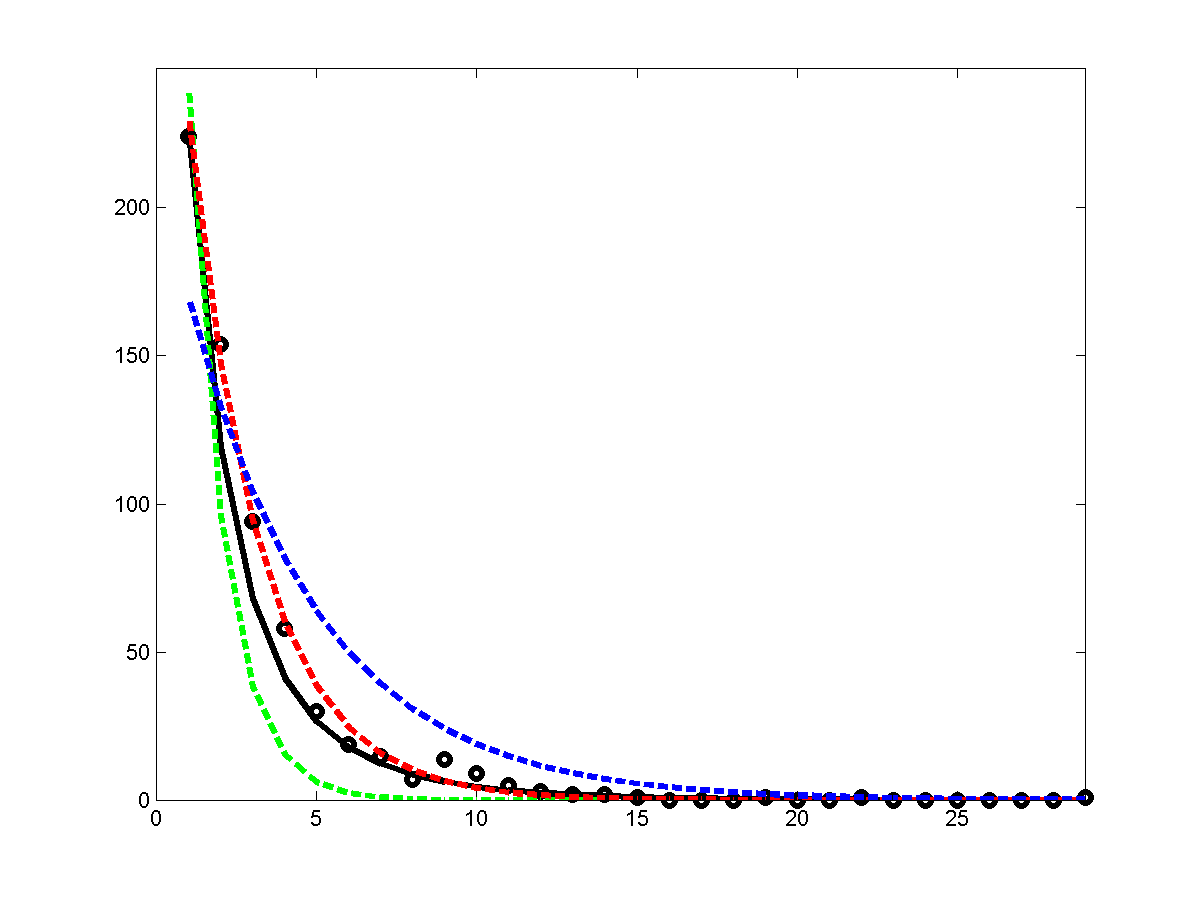
\epsfig{file=../Figures/SimMixtGeomComp.eps, 
       width=.45\textwidth, 4=.height\textheight, clip=} 
    \end{tabular}
  \end{tabular}

  }

%====================================================================
\section{Bayesian Inference}
\frame{ \frametitle{Bayesian Inference}}
%==================================================================== 

%==================================================================== 
\subsection{Mixture models}
\frame{ \frametitle{Inference}
%==================================================================== 
  \paragraph{Inference on truncated data:} 
  \begin{itemize}
  \item Inference of \emphase{mixture of truncated}
    \eqref{Eq:TruncMixt} is often easier than this of
    \emphase{truncated mixture} \eqref{Eq:MixtTrunc}.
  \item MLE estimates for \eqref{Eq:TruncMixt} and
    \eqref{Eq:MixtTrunc} are equivalent (\refer{BoK06}) in the Poisson
    case.
%   \item Truncated geometric $\Gcal$ are still geometric, whereas
%     truncated Poisson $\Pcal$ are not Poisson.
%   \item Precision of the estimates are not that easy to derive in the
%     frequentist context.
  \end{itemize}
  %\refer{BoK06,BeF08,DoB08,HDP10,SHB08}

  \bigskip\pause
  \paragraph{Bayesian inference}
  \begin{itemize}
  \item Bayesian inference provides \emphase{credibility interval}
    through the posterior $P(\thetabf|\Xbf)$.
  \item Exact Bayesian inference with incomplete data requires
    \emphase{computationally intensive MCMC}.
  \item \paragraph{Variational Bayes} provides an (optimal)
    approximation of the joint posterior $P(\thetabf, \Zbf|\Xbf)$ .
%     as
%     $$
%     Q^*(\thetabf, \Zbf) = \underset{Q \in \Qcal}{\arg\min} \;
%     KL\left[Q^*(\thetabf, \Zbf), P(\thetabf, \Zbf|\Xbf) \right]
%     $$
%     in the context of the exponential family with conjugate priors.
  \end{itemize}

  }

%====================================================================
\subsection{Variational Bayes}
%====================================================================
\frame{ \frametitle{Exponential family / Conjugate prior}

  \paragraph{Exponential family:}
  $$
  P(\Xbf, \Zbf|\thetabf) \propto \exp[\emphase{\psi(\thetabf)}' \ubf(\Xbf,
  \Zbf)]
  $$
  includes distributions like geometric, Poisson, truncated
  geometric ... but \emphase{not truncated Poisson} (while they can
  still be handled...)

  \bigskip\pause
  \paragraph{Conjugate prior.}
  $$
  P(\thetabf) \propto \exp[\emphase{\psi(\thetabf)}' \nubf] 
  $$
  that is 
  \begin{itemize}
  \item Dirichlet for the multinomial distribution ($\Zbf$), 
  \item Gamma for Poisson or Beta for the geometric ($\Xbf|\Zbf$),
  \end{itemize}
  $$
  \Rightarrow \qquad P(\thetabf|\Xbf, \Zbf) \propto
  \exp\{\emphase{\psi(\thetabf)}' [\ubf(\Xbf, \Zbf) + \nubf] \}.
  $$

  }

%====================================================================
\frame{ \frametitle{Variational Bayes E-M}

  \paragraph{Best approximation.} As $P(\thetabf, \Zbf|\Xbf)$ is
  intractable, we look for the best 'manageable' approximation:
  \begin{eqnarray*}
    Q^*(\thetabf, \Zbf) & = & \underset{Q \in \Qcal}{\arg\min} \;
    \emphase{KL}[\emphase{Q(\Zbf, \thetabf)}; \emphase{P(\Zbf,
    \thetabf|\Xbf)}] \\ 
    & = & \underset{Q \in \Qcal}{\arg\min} \; \Hcal(\emphase{Q}) -
    \Esp_{\emphase{Q}} [\log \emphase{P(\Xbf, \Zbf, \thetabf)}] + \text{cst}
  \end{eqnarray*}

  \bigskip\bigskip\pause
  \paragraph{Factorisable distributions.} When considering the class
  $$
  \Qcal = \{Q(\thetabf, \Zbf) = \emphase{\Qt(\theta)
    \QZ(\Zbf)}\}, 
  $$
  the optimal $Q^* \in \Qcal$ can be recovered \pause via
  \begin{eqnarray*}
    \text{'M'-step:} \quad \Qt(\thetabf) 
    & \propto 
    & \exp \left(\phi(\thetabf)'
      \left[ \Esp_{\emphase{\QZ}}u(\Xbf, \Zbf) + \nubf \right]
    \right) \\ 
    \\
    \text{'E'-step:} \quad \QZ(\Zbf)     
    & \propto     
    & \exp ( \Esp_{\emphase{\Qt}}\phi(\thetabf)' u(\Xbf, \Zbf) ]
  \end{eqnarray*}
  \refer{BeG03}

  }

%====================================================================
\subsection{Bayesian model averaging}
\frame{ \frametitle{Bayesian model averaging}
%==================================================================== 

  \paragraph{Number of components.} 
  \begin{itemize}
  \item The number of components \emphase{$K$ is unknown} 
  \item ... but the existence of a '\emphase{true}' number of
    component is \emphase{questionable}.
  \end{itemize}
  
  \bigskip\pause
  \paragraph{Bayesian model averaging (BMA).} Instead of choosing the
  'best' $K$ we rather
  \begin{enumerate}
  \item fit the model for a series of $K = 1 \dots K_{\max}$:
    $$
    \Qt^*(\thetabf|K) \approx P(\thetabf | \Xbf, K)
    $$
  \item and then \emphase{average all models} with weights 
    $w_1, \dots w_{K_{\max}}$.
  \end{enumerate}
  
  \bigskip\bigskip\pause
  Standard Bayesian reasoning indicates that the weights should be
  $$
  \emphase{w_K = P(K|\Xbf)}
  $$
  the calculation of which \emphase{remains an issue}.
  
  }

%====================================================================
\frame{ \frametitle{Evaluating the weights}

  \paragraph{Theoretical weights.} We should compute
  $$
  w_K = P(K|\Xbf) \propto P(\Xbf| K) = \frac{P(\Xbf|\thetabf, K)
    P(\thetabf|K)}{\emphase{P(\thetabf|X, K)}}
  $$
  which has no close-form, but a \emphase{plug-in} estimate is
  straightforward:
  $$
  \widehat{w}_K  \propto \frac{P(\Xbf|\thetabf,
    K) P(\thetabf|K)}{\emphase{\Qt^*(\thetabf | K)}}
  $$

  \bigskip\pause
  \paragraph{Optimal variational approximation.} Optimal weights can
  be obtained by direct minimisation of
  $$
  KL[Q(\emphase{K, \Zbf, \thetabf}), P(\emphase{K, \Zbf, \thetabf} | \Xbf)]
  $$
  to get (\Refer{Volant \& al.})
  $$
  \tilde{w}_K := Q^*(K) \propto P(K) \exp\left\{-KL[Q^*(\Zbf,
    \thetabf|K); P(\Zbf, \thetabf|\Xbf, K)] + \log P(\Xbf|K)\right\}.
  $$

  }

%====================================================================
\subsection{Microbial diversity in human gut}
\frame{ \frametitle{Microbial diversity in human gut (\refer{TML09})}
%==================================================================== 

  \paragraph{Fit of different geometric mixtures $K = 1, \dots 5$:}
  $\widehat{\thetabf}_K =$ mode of $\Qt(\thetabf)$.
  $$
  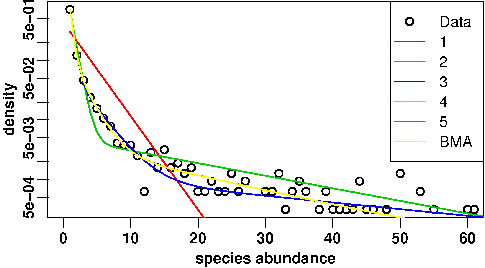
\epsfig{file=../Figures/TapMondot2.eps, width=0.75\textwidth, clip=}
  $$
  $$
  \emphase{\text{Mixture: }} \widehat{f}^K_+(x) = \sum_k
    \widehat{\pi}_K \phi_+(x; \widehat{\gamma}_K), 
  \qquad
  \emphase{\text{BMA: }} \widetilde{f}_+(x) = \sum_K w_K \widehat{f}^K_+(x). 
  $$

  }

%==================================================================== 
\frame{ \frametitle{Saturation curve}

  \paragraph{Reverse use of $\widetilde{f}_+(x)$:} Design of NGS
  metagenomics experiment
  $$
  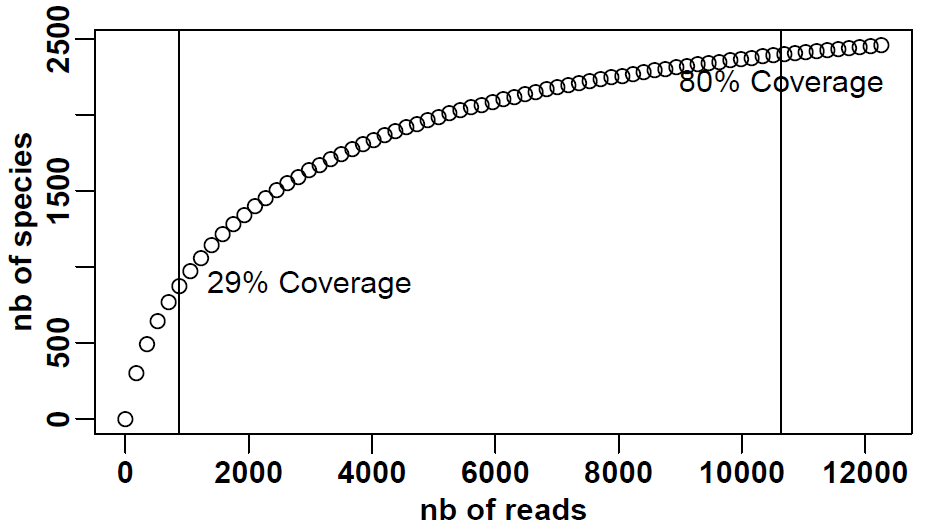
\epsfig{file=../Figures/Rarefaction.ps, width=0.75\textwidth, clip=}
  $$

  }

%====================================================================
\section{Confidence interval for the number of species}
\frame{ \frametitle{Confidence interval for the number of species}}
%====================================================================

%====================================================================
\subsection{Estimation of the total number of species}
\frame{ \frametitle{Estimation of the total number of species}
%==================================================================== 

  \paragraph{Geometric distribution.} The proportion of absent species
  under the geometric distribution is
  $$
  \widehat{\phi}(0) = \widehat{\gamma}
  $$
  for which the \emphase{approximate posterior $Q^*_K(\gamma)$ is a
    Beta distribution}.

  \bigskip\pause
  \paragraph{Mixture of geometric,} we get
  $$
  \widehat{f}_K(0) = \sum_k \widehat{\pi}_{k=1}^K \widehat{\gamma}_k.
  $$

  \bigskip\pause
  \paragraph{Number of absent species.} The Horwitz-Thomson is
  $$
  \widehat{C}_K = c / [1 - \widehat{f}_K(0)].
  $$

  \bigskip
  \paragraph{BMA} can also be applied:
  $$
  \widetilde{C} = \sum_{K=1}^{K_{\max}} w_K \widehat{C}_K.
  $$

  }

%====================================================================
\subsection{Importance sampling}
\frame{ \frametitle{Importance sampling}
%==================================================================== 

  \paragraph{Approximate posterior.} 
  \begin{itemize}
  \item Variational Bayes only provides an \emphase{approximate
      posterior $\Qt(\thetabf)$}.
  \item which is known to often \emphase{under-estimate} the posterior
    variances.
  \end{itemize}

  \bigskip\pause
  \paragraph{Monte-Carlo estimate.} Taking \emphase{$(\thetabf^b)_b \text{
      i.i.d.} \sim P(\thetabf)$}, we have
  $$
  \int_{\Ical} P(\Xbf|\thetabf) P(\thetabf) \dd \thetabf
  \simeq 
  \frac1B \sum_{\thetabf^b \in \Ical} P(\Xbf|\thetabf^b) 
  =: 
  \widehat{P}(\thetabf \in \Ical|\Xbf) 
  $$
  but the variance is large when $P(\thetabf)$ is \emphase{far from}
  $P(\thetabf|\Xbf)$.
    
  \bigskip\pause
  \paragraph{Importance sampling (IS)} provides smaller
  variance with \emphase{$(\thetabf^b)_b \sim Q(\thetabf)$}
  $$
  \int_{\Ical} P(\Xbf|\thetabf)
  \emphase{\frac{P(\thetabf)}{Q(\thetabf)}} Q(\thetabf) \dd \thetabf
  \simeq \frac1B \sum_{\thetabf^b \in \Ical}
  \emphase{\frac{P(\thetabf^b)}{Q(\thetabf^b)}} P(\Xbf|\thetabf^b) =:
  \widehat{P}(\thetabf \in \Ical|\Xbf)
%   \frac1{P(\Xbf)} \int P(\Xbf|\thetabf) \frac{P(\Xbf)}{Q(\Xbf)}
%   Q(\thetabf) \dd \thetabf \simeq \frac1B \sum_b P(\Xbf|\thetabf^b)
%   \frac{P(\Xbf)}{Q(\Xbf)} =: \widehat{P}(\thetabf|\Xbf).
  $$
  \emphase{$\Qt^*(\thetabf)$ is a good proxy} of $P(\thetabf|\Xbf)$. 
    
  }

%====================================================================
\frame{ \frametitle{Approximate posterior distribution}
  
  A Gibbs sampler (\textcolor{blue}{MCMC}) is
  used as a \emphase{gold standard for $\widehat{P}(X|\Xbf)$}. \\
  \bigskip
  \begin{tabular}{cc}
    \begin{tabular}{c}
      \paragraph{Simulated data:} $f_+(0)$ \vspace{.15cm} \\      
      \epsfig{file=../Figures/VBEM3.eps, width=0.45\textwidth,
        height=0.325\textwidth} \pause 
    \end{tabular} 
    &
    \begin{tabular}{c}
      \paragraph{Human gut:} $C_0$ \\
      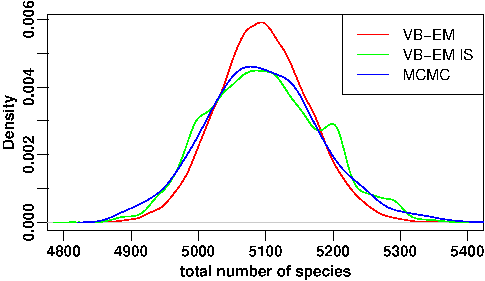
\epsfig{file=../Figures/VBEM4.eps, width=0.45\textwidth,
        height=0.375\textwidth} 
    \end{tabular}
  \end{tabular}

  \bigskip
  \begin{itemize}
  \item \vspace{-.5cm} \textcolor{red}{VB-EM} under-estimates the
    posterior variability.
  \item \textcolor{green}{IS} provides a better estimates, with similar
    credibility intervals.
  \end{itemize}
  }

%====================================================================
\section{Conclusion}
\frame{ \frametitle{Conclusion \& Future works}
%==================================================================== 

  \paragraph{Species abundance} is an old statistical problem
  revisited by metagenomics.

  \bigskip
  \paragraph{Mixture models} provide a flexible modelling of the
  species abundance distribution (SAD).

  \bigskip\pause
  \paragraph{Variational Bayes Model Averaging} 
  \begin{itemize}
  \item allows to get a \emphase{good approximation of the posterior}
    distribution of the parameter of interest
  \item and can be \emphase{further improved by importance sampling}, which is
    still less computationally demanding than regular MCMC.
  \end{itemize}

  \bigskip\pause
  \paragraph{A true non-parametric estimate of the SAD} 
  can be considered, under mild restriction such as convexity.

  \bigskip
  {\centerline{
    \textcolor{blue}{SMPGD'10: 27-28 in January at Institut Curie (Paris)}
    }}
  
  }

%====================================================================
{\tiny
  \bibliography{/Biblio/AST,/Biblio/ARC,/Biblio/SSB}
  \bibliographystyle{/Latex/astats}
  %\bibliographystyle{plain}
  }

%====================================================================
%====================================================================
\end{document}
%====================================================================
%====================================================================

  \begin{tabular}{cc}
    \hspace{-.5cm}
    \begin{tabular}{p{.5\textwidth}}
    \end{tabular}
    & 
    \hspace{-.5cm}
    \begin{tabular}{p{.5\textwidth}}
    \end{tabular}
  \end{tabular}

